\subsubsection{Prvo, pa 1}

\def\fibonacci#1#2#3{%
\newcount\o \o=#1
\newcount\t \t=#2
\number\o,~\number\t
\newcount\f
\newcount\n \n=#3 \advance\n-2
\loop
  \f=\t \advance\t\o \o=\f
  , \number\t
  \advance \n -1
\ifnum \n>0 \repeat}

\zadatak 
Koliki procenat cena {\sl od igle do lokomotive\/}
% Koliki procenat {\sl Fibona{\cv}ijevih brojeva\/} (Leonardo Bonacci) \fibonacci11{25},~\dots\
po{\cv}i{\nj}e cifrom~1?

\resenje Iz formule \eqref{eq:benford} sa strane \pageref{eq:benford} sledi da je $p_1=\logten 2 \approx \ram{30\%}$.

\dodatak Ovu zakonitost je prvi otkrio 1881.\ astronom {\Nj}ucom (Simon Newcomb), kada je primetio da su
listovi logaritamskih tablica koje je dugo koristio najpr{\lj}aviji
na po{\cv}etku: 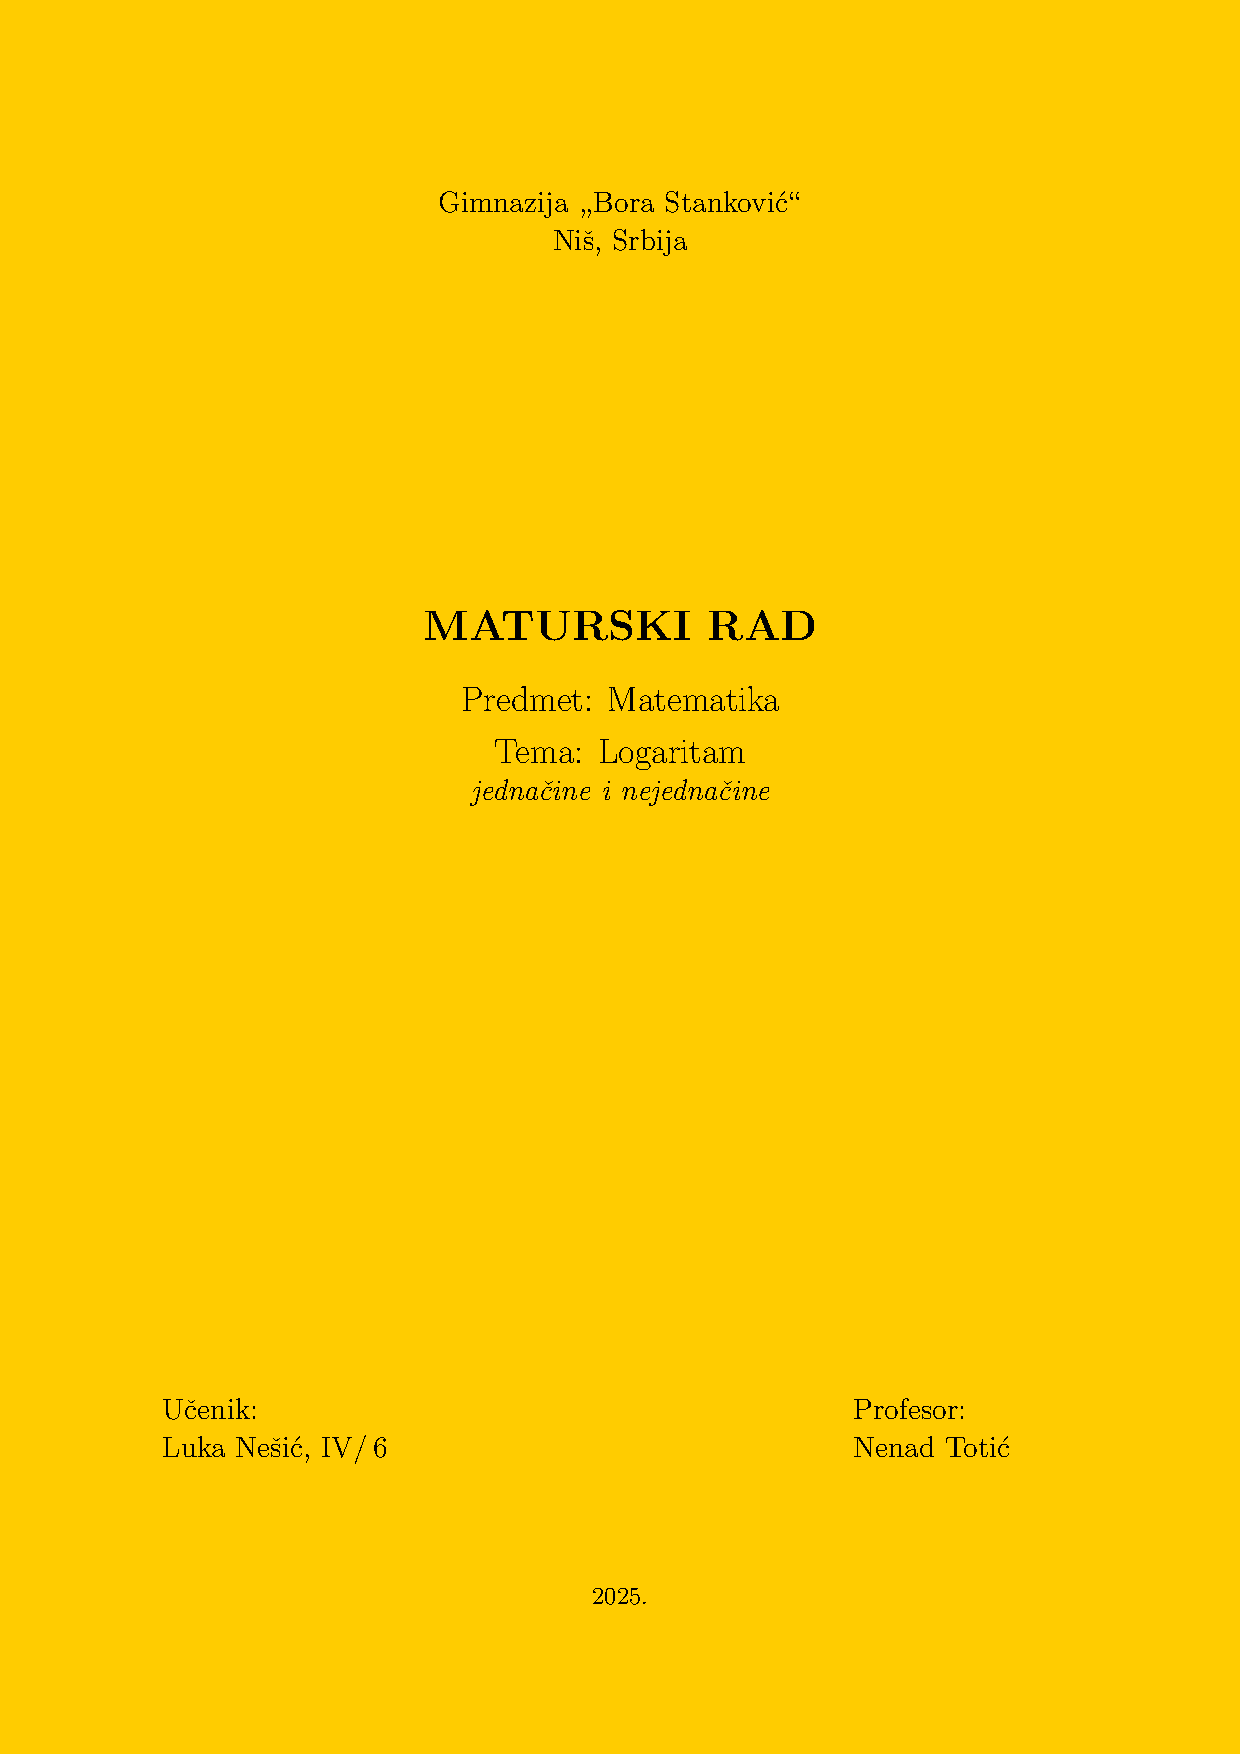
\includegraphics{log.4}.
